\def\paperversiondraft{draft}
\def\paperversionblind{normal}
\def\paperversioncameraIEEE{cameraIEEE}

% If no draft paper-version is requested, compile in 'normal' mode
\ifx\paperversion\paperversiondraft
\else
  \ifx\paperversion\paperversioncameraIEEE
  \else
    \def\paperversion{normal}
  \fi
\fi

\def\grammarlyon{on}

% Disable review mode for grammarly version.
\ifx\grammarly\grammarlyon
\def\ClassReview{}
\else
\def\ClassReview{review,}
\fi

\ifx\paperversion\paperversioncameraIEEE
  \documentclass[conference]{IEEEtran}
\else
  \documentclass[\ClassReview anonymous, sigplan]{acmart}
\fi

\def\acmversionanonymous{anonymous}
\def\acmversionjournal{journal}
\def\acmversionnone{none}

\ifx\paperversion\paperversioncameraIEEE
    \def\acmversion{none}
\else
  \makeatletter
  \if@ACM@anonymous
    \def\acmversion{anonymous}
  \else
    \def\acmversion{journal}
  \fi
  \makeatother
\fi

\usepackage{colortbl}

% 'draftonly' environment
\usepackage{environ}
\ifx\paperversion\paperversiondraft
\newenvironment{draftonly}{}{}
\else
\NewEnviron{draftonly}{}
\fi

% Most PL conferences are edited by conference-publishing.com. Follow their
% advice to add the following packages.
%
% The first enables the use of UTF-8 as character encoding, which is the
% standard nowadays. The second ensures the use of font encodings that support
% accented characters etc. (Why should I use this?). The mictotype package
% enables certain features 'to­wards ty­po­graph­i­cal per­fec­tion
\usepackage[utf8]{inputenc}
\usepackage[T1]{fontenc}
\usepackage{microtype}

\usepackage{minted}
\usemintedstyle{colorful}
\newminted[mlir]{tools/MLIRLexer.py:MLIRLexerOnlyOps -x}{mathescape}

\usepackage{xargs}
\usepackage{lipsum}
\usepackage[textsize=tiny]{todonotes}
\usepackage{xparse}
\usepackage{xifthen, xstring}
\usepackage[normalem]{ulem}
\usepackage{xspace}
\usepackage{marginnote}
\usepackage{etoolbox}

\makeatletter
\font\uwavefont=lasyb10 scaled 652

\newcommand\colorwave[1][blue]{\bgroup\markoverwith{\lower3\p@\hbox{\uwavefont\textcolor{#1}{\char58}}}\ULon}
\makeatother

\ifx\paperversion\paperversiondraft
\newcommand\createtodoauthor[2]{%
\def\tmpdefault{emptystring}
\expandafter\newcommand\csname #1\endcsname[2][\tmpdefault]{\def\tmp{##1}\ifthenelse{\equal{\tmp}{\tmpdefault}}
   {\todo[linecolor=#2,backgroundcolor=#2,bordercolor=#2]{\textbf{#1:} ##2}}
   {\ifthenelse{\equal{##2}{}}{\colorwave[#2]{##1}\xspace}{\todo[linecolor=#2,backgroundcolor=#2,bordercolor=#2]{\textbf{#1:} ##2}\colorwave[#2]{##1}}}}
\expandafter\newcommand\csname #1f\endcsname[2][\tmpdefault]{
	\smash{\marginnote{
		\todo[inline,linecolor=#2,backgroundcolor=#2,bordercolor=#2]{\textbf{#1 (Figure):} ##2}}}
   }
}
%
\else
\newcommand\createtodoauthor[2]{%
\expandafter\newcommand\csname #1\endcsname[2][]{##1}%
\expandafter\newcommand\csname #1f\endcsname[2][]{##1}%
}%
\fi

% Broaden margins to make room for todo notes
\makeatletter
\patchcmd{\@addmarginpar}{\ifodd\c@page}{\ifodd\c@page\@tempcnta\m@ne}{}{}
\makeatother
\ifx\paperversion\paperversiondraft
  \ifx\acmversion\acmversionjournal
    \geometry{asymmetric}
    \paperwidth=\dimexpr \paperwidth + 3.5cm\relax
    \oddsidemargin=\dimexpr\oddsidemargin + 0cm\relax
    \evensidemargin=\dimexpr\evensidemargin + 0cm\relax
    \marginparwidth=\dimexpr \marginparwidth + 3cm\relax
    \setlength{\marginparwidth}{4.6cm}
    % This makeatletter box helps to move notes to the right
    \makeatletter
    \long\def\@mn@@@marginnote[#1]#2[#3]{%
      \begingroup
        \ifmmode\mn@strut\let\@tempa\mn@vadjust\else
          \if@inlabel\leavevmode\fi
          \ifhmode\mn@strut\let\@tempa\mn@vadjust\else\let\@tempa\mn@vlap\fi
        \fi
        \@tempa{%
          \vbox to\z@{%
            \vss
            \@mn@margintest
            \if@reversemargin\if@tempswa
                \@tempswafalse
              \else
                \@tempswatrue
            \fi\fi
            %\if@tempswa
              \rlap{%
                \if@mn@verbose
                  \PackageInfo{marginnote}{xpos seems to be \@mn@currxpos}%
                \fi
                \begingroup
                  \ifx\@mn@currxpos\relax\else\ifx\@mn@currxpos\@empty\else
                      \kern-\dimexpr\@mn@currxpos\relax
                  \fi\fi
                  \ifx\@mn@currpage\relax
                    \let\@mn@currpage\@ne
                  \fi
                  \if@twoside\ifodd\@mn@currpage\relax
                      \kern\oddsidemargin
                    \else
                      \kern\evensidemargin
                    \fi
                  \else
                    \kern\oddsidemargin
                  \fi
                  \kern 1in
                \endgroup
                \kern\marginnotetextwidth\kern\marginparsep
                \vbox to\z@{\kern\marginnotevadjust\kern #3
                  \vbox to\z@{%
                    \hsize\marginparwidth
                    \linewidth\hsize
                    \kern-\parskip
                    \marginfont\raggedrightmarginnote\strut\hspace{\z@}%
                    \ignorespaces#2\endgraf
                    \vss}%
                  \vss}%
              }%
          }%
        }%
      \endgroup
    }
    \makeatother
  \else
    \paperwidth=\dimexpr \paperwidth + 6cm\relax
    \oddsidemargin=\dimexpr\oddsidemargin + 3cm\relax
    \evensidemargin=\dimexpr\evensidemargin + 3cm\relax
    \marginparwidth=\dimexpr \marginparwidth + 3cm\relax
    \setlength{\marginparwidth}{4.6cm}
  \fi
\fi

% We use the following color scheme
% 
% This scheme is both print-friendly and colorblind safe for
% up to four colors (including the red tones makes it not
% colorblind safe any more)
%
% https://colorbrewer2.org/#type=qualitative&scheme=Paired&n=4

\definecolor{pairedNegOneLightGray}{HTML}{cacaca}
\definecolor{pairedNegTwoDarkGray}{HTML}{827b7b}
\definecolor{pairedOneLightBlue}{HTML}{a6cee3}
\definecolor{pairedTwoDarkBlue}{HTML}{1f78b4}
\definecolor{pairedThreeLightGreen}{HTML}{b2df8a}
\definecolor{pairedFourDarkGreen}{HTML}{33a02c}
\definecolor{pairedFiveLightRed}{HTML}{fb9a99}
\definecolor{pairedSixDarkRed}{HTML}{e31a1c}

\definecolor{mygreen}{rgb}{0,0.6,0}
%% Some colors for the polts (color blind safe)
%% https://www.acm.org/publications/proceedings-template
%% note RGB if you want to put the color in decimal.
%% color scheme: 3 colors
\definecolor{blind_safe_one_scheme_three_colors}{RGB}{102,194,165}
\definecolor{blind_safe_two_scheme_three_colors}{RGB}{252,141,98}
\definecolor{blind_safe_three_scheme_three_colors}{RGB}{141,160,203}
%% color scheme: 4 colors
\definecolor{blind_safe_one_scheme_four_colors}{RGB}{166,206,227}
\definecolor{blind_safe_two_scheme_four_colors}{RGB}{31,120,180} 
\definecolor{blind_safe_three_scheme_four_colors}{RGB}{178,223,138}
\definecolor{blind_safe_four_scheme_four_colors}{RGB}{51,160,44}
%% color scheme: 7 colors
\definecolor{blind_safe_one_scheme_seven_colors}{RGB}{118,42,131}
\definecolor{blind_safe_two_scheme_seven_colors}{RGB}{175,141,195}
\definecolor{blind_safe_three_scheme_seven_colors}{RGB}{231,212,232}
\definecolor{blind_safe_four_scheme_seven_colors}{RGB}{247,247,247}
\definecolor{blind_safe_five_scheme_seven_colors}{RGB}{217,240,211}
\definecolor{blind_safe_six_scheme_seven_colors}{RGB}{127,191,123}
\definecolor{blind_safe_seven_scheme_seven_colors}{RGB}{27,120,55}

\definecolor{butter1}{rgb}{0.988,0.914,0.310}
\definecolor{butter2}{rgb}{0.929,0.831,0.000}
\definecolor{butter3}{rgb}{0.769,0.627,0.000}

\definecolor{orange1}{rgb}{0.988,0.686,0.243}
\definecolor{orange2}{rgb}{0.961,0.475,0.000}
\definecolor{orange3}{rgb}{0.808,0.361,0.000}

\definecolor{chocolate1}{rgb}{0.914,0.725,0.431}
\definecolor{chocolate2}{rgb}{0.757,0.490,0.067}
\definecolor{chocolate3}{rgb}{0.561,0.349,0.008}

\definecolor{chameleon1}{rgb}{0.541,0.886,0.204}
\definecolor{chameleon2}{rgb}{0.451,0.824,0.086}
\definecolor{chameleon3}{rgb}{0.306,0.604,0.024}

\definecolor{skyblue1}{rgb}{0.447,0.624,0.812}
\definecolor{skyblue2}{rgb}{0.204,0.396,0.643}
\definecolor{skyblue3}{rgb}{0.125,0.290,0.529}

\definecolor{plum1}{rgb}{0.678,0.498,0.659}
\definecolor{plum2}{rgb}{0.459,0.314,0.482}
\definecolor{plum3}{rgb}{0.361,0.208,0.400}

\definecolor{scarletred1}{rgb}{0.937,0.161,0.161}
\definecolor{scarletred2}{rgb}{0.800,0.000,0.000}
\definecolor{scarletred3}{rgb}{0.643,0.000,0.000}

\definecolor{aluminium1}{rgb}{0.933,0.933,0.925}
\definecolor{aluminium2}{rgb}{0.827,0.843,0.812}
\definecolor{aluminium3}{rgb}{0.729,0.741,0.714}
\definecolor{aluminium4}{rgb}{0.533,0.541,0.522}
\definecolor{aluminium5}{rgb}{0.333,0.341,0.325}
\definecolor{aluminium6}{rgb}{0.180,0.204,0.212}

\createtodoauthor{grosser}{pairedOneLightBlue}
\createtodoauthor{authorTwo}{pairedTwoDarkBlue}
\createtodoauthor{authorThree}{pairedThreeLightGreen}
\createtodoauthor{authorFour}{pairedFourDarkGreen}
\createtodoauthor{authorFive}{pairedFiveLightRed}
\createtodoauthor{authorSix}{pairedSixDarkRed}

\graphicspath{{./images/}}

% Define macros that are used in this paper
%
% We require all macros to end with a delimiter (by default {}) to enusure
% that LaTeX adds whitespace correctly.
\makeatletter
\newcommand\requiredelimiter[2][########]{%
  \ifdefined#2%
    \def\@temp{\def#2#1}%
    \expandafter\@temp\expandafter{#2}%
  \else
    \@latex@error{\noexpand#2undefined}\@ehc
  \fi
}
\@onlypreamble\requiredelimiter
\makeatother

\newcommand\newdelimitedcommand[2]{
\expandafter\newcommand\csname #1\endcsname{#2}
\expandafter\requiredelimiter
\csname #1 \endcsname
}

\newdelimitedcommand{toolname}{Tool}


% Print \autoref as "Section X.Y.Z"
\ifx\paperversion\paperversioncameraIEEE
\else
  \renewcommand*{\sectionautorefname}{Section}
  \renewcommand*{\subsectionautorefname}{Section}
  \renewcommand*{\subsubsectionautorefname}{Section}
\fi

% \circled command to print a colored circle.
% \circled{1} pretty-prints "(1)"
% This is useful to refer to labels that are embedded within figures.
\usepackage{tikz}
\usetikzlibrary{arrows}
\usetikzlibrary{shapes}
\DeclareRobustCommand\circled[2][]{\ifthenelse{\isempty{#1}}{\tikz[baseline=(char.base)]{\node[shape=circle,fill=pairedOneLightBlue,inner sep=1pt] (char) {#2};}}{\autoref{#1}: \hyperref[#1]{\tikz[baseline=(char.base)]{\node[shape=circle,fill=pairedOneLightBlue,inner sep=1pt] (char) {#2};}}}}


\ifx\paperversion\paperversioncameraIEEE
\else
  \ifx\acmversion\acmversionjournal
  %% Journal information (used by PACMPL format)
  %% Supplied to authors by publisher for camera-ready submission
  \acmJournal{PACMPL}
  \acmVolume{1}
  \acmNumber{1}
  \acmArticle{1}
  \acmYear{2017}
  \acmMonth{1}
  \acmDOI{10.1145/nnnnnnn.nnnnnnn}
  \startPage{1}
  \else
  %% Conference information (used by SIGPLAN proceedings format)
  %% Supplied to authors by publisher for camera-ready submission
  \acmConference[PL'17]{ACM SIGPLAN Conference on Programming Languages}{January 01--03, 2017}{New York, NY, USA}
  \acmYear{2017}
  \acmISBN{978-x-xxxx-xxxx-x/YY/MM}
  \acmDOI{10.1145/nnnnnnn.nnnnnnn}
  \startPage{1}
  \fi
\fi


%% Copyright information
%% Supplied to authors (based on authors' rights management selection;
%% see authors.acm.org) by publisher for camera-ready submission
%\setcopyright{none}             %% For review submission
%\setcopyright{acmcopyright}
%\setcopyright{acmlicensed}
%\setcopyright{rightsretained}
%\copyrightyear{2017}           %% If different from \acmYear


%% Bibliography style
\ifx\paperversion\paperversioncameraIEEE
  \bibliographystyle{IEEETran}
\else
  \bibliographystyle{ACM-Reference-Format}
\fi
%% Citation style
%% Note: author/year citations are required for papers published as an
%% issue of PACMPL.
%\citestyle{acmauthoryear}  %% For author/year citations
%\citestyle{acmnumeric}     %% For numeric citations
%\setcitestyle{nosort}      %% With 'acmnumeric', to disable automatic
                            %% sorting of references within a single citation;
                            %% e.g., \cite{Smith99,Carpenter05,Baker12}
                            %% rendered as [14,5,2] rather than [2,5,14].
%\setcitesyle{nocompress}   %% With 'acmnumeric', to disable automatic
                            %% compression of sequential references within a
                            %% single citation;
                            %% e.g., \cite{Baker12,Baker14,Baker16}
                            %% rendered as [2,3,4] rather than [2-4].



\begin{document}

%% Title information
\ifx\paperversion\paperversioncameraIEEE
  \title{Full title}
\else
  \title[]{MOM: Matrix Operations in MLIR}       %% [Short Title] is optional;
                                        %% when present, will be used in
                                        %% header instead of Full Title.
  \subtitle{Compiler Support for Linear-algebra Computations in MLIR} %% \subtitle is optional
\fi


%% Author information
%% Contents and number of authors suppressed with 'anonymous'.
%% Each author should be introduced by \author, followed by
%% \authornote (optional), \orcid (optional), \affiliation, and
%% \email.
%% An author may have multiple affiliations and/or emails; repeat the
%% appropriate command.
%% Many elements are not rendered, but should be provided for metadata
%% extraction tools.

%% Author with single affiliation.
\ifx\paperversion\paperversioncameraIEEE
  \author{\IEEEauthorblockN{1\textsuperscript{st} Given Name Surname}
  \IEEEauthorblockA{\textit{dept. name of organization (of Aff.)} \\
  \textit{name of organization (of Aff.)}\\
  City, Country \\
  email address or ORCID}
  \and
  \IEEEauthorblockN{2\textsuperscript{nd} Given Name Surname}
  \IEEEauthorblockA{\textit{dept. name of organization (of Aff.)} \\
  \textit{name of organization (of Aff.)}\\
  City, Country \\
  email address or ORCID}
  \and
  \IEEEauthorblockN{3\textsuperscript{rd} Given Name Surname}
  \IEEEauthorblockA{\textit{dept. name of organization (of Aff.)} \\
  \textit{name of organization (of Aff.)}\\
  City, Country \\
  email address or ORCID}
  \and
  \IEEEauthorblockN{4\textsuperscript{th} Given Name Surname}
  \IEEEauthorblockA{\textit{dept. name of organization (of Aff.)} \\
  \textit{name of organization (of Aff.)}\\
  City, Country \\
  email address or ORCID}
  \and
  \IEEEauthorblockN{5\textsuperscript{th} Given Name Surname}
  \IEEEauthorblockA{\textit{dept. name of organization (of Aff.)} \\
  \textit{name of organization (of Aff.)}\\
  City, Country \\
  email address or ORCID}
  \and
  \IEEEauthorblockN{6\textsuperscript{th} Given Name Surname}
  \IEEEauthorblockA{\textit{dept. name of organization (of Aff.)} \\
  \textit{name of organization (of Aff.)}\\
  City, Country \\
  email address or ORCID}
  }
\else
  \author{First1 Last1}
  \authornote{with author1 note}          %% \authornote is optional;
                                        %% can be repeated if necessary
  \orcid{nnnn-nnnn-nnnn-nnnn}             %% \orcid is optional
  \affiliation{
    \position{Position1}
    \department{Department1}              %% \department is recommended
    \institution{Institution1}            %% \institution is required
    \streetaddress{Street1 Address1}
    \city{City1}
    \state{State1}
    \postcode{Post-Code1}
    \country{Country1}
  }
  \email{first1.last1@inst1.edu}          %% \email is recommended

  \author{First2 Last2}
  \authornote{with author2 note}          %% \authornote is optional;
                                        %% can be repeated if necessary
  \orcid{nnnn-nnnn-nnnn-nnnn}             %% \orcid is optional
  \affiliation{
    \position{Position2a}
    \department{Department2a}             %% \department is recommended
    \institution{Institution2a}           %% \institution is required
    \streetaddress{Street2a Address2a}
    \city{City2a}
    \state{State2a}
    \postcode{Post-Code2a}
    \country{Country2a}
  }
  \email{first2.last2@inst2a.com}         %% \email is recommended
  \affiliation{
    \position{Position2b}
    \department{Department2b}             %% \department is recommended
    \institution{Institution2b}           %% \institution is required
    \streetaddress{Street3b Address2b}
    \city{City2b}
    \state{State2b}
    \postcode{Post-Code2b}
    \country{Country2b}
  }
  \email{first2.last2@inst2b.org}         %% \email is recommended
\fi

\def\makeabstract{
\begin{abstract}
% An abstract should consist of six main sentences:
%  1. Introduction. In one sentence, what’s the topic?
%  2. State the problem you tackle.
%  3. Summarize (in one sentence) why nobody else has adequately answered the research question yet.
%  4. Explain, in one sentence, how you tackled the research question.
%  5. In one sentence, how did you go about doing the research that follows from your big idea.
%  6. As a single sentence, what’s the key impact of your research?

% (http://www.easterbrook.ca/steve/2010/01/how-to-write-a-scientific-abstract-in-six-easy-steps/)

  Dense linear algebra arises in numerical software in computational science
  and engineering. Often computations in dense linear algebra rely on
  highly-optimized building blocks from libraries such as BLAS and LAPACK.
  While such libraries provide portable performance for a wide range of
  computing architectures, they still present limitations in terms of
  flexibility. In this paper, we propose a new MLIR dialect for expressing
  linear algebraic computations and their optimization starting from properties
  of the matrices contained in the input expressions (e.g., their matrix
  structure).  The integration of this new dialect in MLIR enables end-to-end
  compilation of matrix computations via conversion to existing lower-level
  dialects already provided by the framework.


%\lipsum[1]
\end{abstract}
}

\ifx\paperversion\paperversioncameraIEEE
\else
  \makeabstract
\fi

% Only add ACM notes and keywords in camera ready version
% Drop citations and footnotes in draft and blind mode.
\ifx\acmversion\acmversionanonymous
\settopmatter{printacmref=false} % Removes citation information below abstract
\renewcommand\footnotetextcopyrightpermission[1]{} % removes footnote with conference information in first column
\fi
\ifx\acmversion\acmversionjournal
%% 2012 ACM Computing Classification System (CSS) concepts
%% Generate at 'http://dl.acm.org/ccs/ccs.cfm'.
\begin{CCSXML}
<ccs2012>
<concept>
<concept_id>10011007.10011006.10011008</concept_id>
<concept_desc>Software and its engineering~General programming languages</concept_desc>
<concept_significance>500</concept_significance>
</concept>
<concept>
<concept_id>10003456.10003457.10003521.10003525</concept_id>
<concept_desc>Social and professional topics~History of programming languages</concept_desc>
<concept_significance>300</concept_significance>
</concept>
</ccs2012>
\end{CCSXML}

\ccsdesc[500]{Software and its engineering~General programming languages}
\ccsdesc[300]{Social and professional topics~History of programming languages}
%% End of generated code

%% Keywords
%% comma separated list
\keywords{keyword1, keyword2, keyword3} 
\fi

%% \maketitle
%% Note: \maketitle command must come after title commands, author
%% commands, abstract environment, Computing Classification System
%% environment and commands, and keywords command.
\maketitle
\ifx\grammarly\grammarlyon 
\onecolumn 
\else 
\fi

% IEEE wants abstract and keywords 
% after maketitle
\ifx\paperversion\paperversioncameraIEEE
  \makeabstract
%% Keywords
%% comma separated list
  \begin{IEEEkeywords}
    keyword1, keyword2, keyword3  %% \keywords is optional
  \end{IEEEkeywords}
\fi

\section{Introduction}

A significant part of processor time is spent on mathematical algorithms used
in simulations, machine learning, communication, signal processing, computer
vision, and other domains. Of course, the mathematics used in these domains may
differ widely. Still, the actual computations often fall into the realm of
linear algebra, meaning sequences of computations on matrices and vectors. 
Research in the area of linear algebraic domain-specific languages (DSLs) have
demonstrated that expert-level optimizations can be carried out automatically
when taking the mathematical semantics of the computation into account (e.g.,
\cite{barthels:21, spampinato:18, kjolstad:17}). Over time, however, the code
generation infrastructure supporting such research has grown into a fragmented
software ecosystem, where different components that could logically cooperate
towards a shared performance goal are in practice unable to interoperate with
one another.

This paper proposes an implementation of a subset of a state-of-the-art
linear-algebra code generator in MLIR. The linear-algebra code-generator is
Linnea~\cite{10.1145/3446632}.  Specifically, our contributions are:

\begin{figure}
% Link to figure
%
% https://docs.google.com/drawings/d/1juKp43D3rLC-luBQPwQZ_wCnDK2S_6C1k6USV0wKE0g/edit?usp=sharing
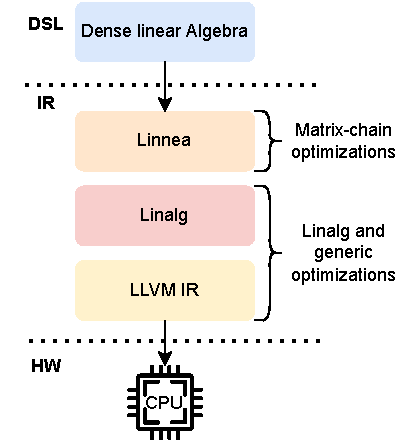
\includegraphics[width=0.6\columnwidth]{images/Impact2022.drawio.pdf}
\caption{The MOM compiler for dense-linear algebra.}
\end{figure}

\begin{itemize}
	\item An IR representation to model linear-algebra operations, types and properties.
	\item A lowering from such representation to LLVM IR.
\end{itemize}

\section{The Linnea Dialect}

Dense linear algebra support is captured in MLIR by introducing a new dialect
called Linnea after the system developed in~\cite{10.1145/3446632}.  The Linnea
dialect provides MLIR attributes, types, operations, and transformations
required to make dense computation as first-class citizens in the compiler IR.
Linnea forms a bridge between the high-level dense linear-algebra mathematics
expressed in a Python DSL and a more BLAS-like dialect: Linalg. From Linalg we
lower to LLVM IR and then machine code.

\paragraph{Matrix Attribute}

\begin{listing}[]
\begin{center}
\begin{minipage}[]{0.5\textwidth}
\begin{minted}[fontsize=\scriptsize, escapeinside=@@]{cpp}
  @\color{orange3}{#linnea.property}@<[@\color{skyblue3}{'lowerTri'}@]>
\end{minted}
\end{minipage}
\caption{Linnea attributes attach properties to the underneath algebraic object.}
\label{lst:attribute}
\end{center}
\end{listing}

Central to the design of our dialect is the \texttt{Matrix} attribute a
notation mechanism -- inspired from the Sparse Tensor Dialect -- to encode
compile-time information that defines a given \texttt{Matrix} type. A
\texttt{Matrix} attribute is thus a list of non-conflicting properties that
define the underneath algebraic object (e.g., lower or upper triangular).
Listing~\ref{lst:attribute} shows an attribute to flag an algebraic type as
lower triangular. During bufferization~\footnote{bufferization materializes
memref (i.e., malloc) from tensors.}, the underneath algebraic object is
materialized using a straightforward \texttt{memref} where attributes dictates
how the memory is filled (i.e., set to zeros the element below the diagonal for
an upper triangular matrix). In the future, we would like to depart from
\texttt{memref} and use more appropriate containers.

\paragraph{Types: Matrix, Term and Identity}

Linnea provides three built-in types: Matrix, Term and Identity. Matrix
represents a specialization of an n-dimensional tensor type that guarantees a
2-dimensional shape. It comes with an attribute that describes a set of
non-conflicting properties, a static dimension, and an MLIR built-in type that
describes each stored element's type (i.e., f32). Listing~\ref{lst:type} shows
how a 5 $\times$ 5 lower-triangular matrix can be represented. A term type
represents the result of Linnea \texttt{equationOp}. It is a placeholder type,
meaning that it will be replaced by a concrete one (i.e., \texttt{MatrixType}).
In fact, only after optimization and simplification the result of an
\texttt{equationOp} is known and thus the placeholder types can be swapped with
a concrete one. Finally, an Identity type represents the identity matrix -- a
square matrix where all the elements on the diagonal are 1. The identity types
can unlock some interesting optimizations, for example: $A * I = A$ or $I * I =
I$.

\begin{listing}[]
\begin{center}
\begin{minipage}[]{0.5\textwidth}
\begin{minted}[fontsize=\scriptsize, escapeinside=@@]{cpp}
  !linnea.matrix@\color{orange3}{#linnea.property}@<[@\color{skyblue3}{'lowerTri'}@, [5, 5], @\color{red}{f32}@]>
\end{minted}
\end{minipage}
  \caption{A type to represent a 5 $\times$ 5 lower-triangular matrix with \texttt{f32} as element type.}
\label{lst:type}
\end{center}
\end{listing}

\paragraph{Operations}

Table shows the operations exposed by the Linnea
dialect~\ref{table:operations}. \texttt{Init} and \texttt{Fill} initialize and
fill an algebraic object, respectively. \texttt{Mul} and \texttt{Add} are
variadic operations that takes as input an arbitrary numbers of Values of
Linnea types.  The \texttt{Equation} represents a ``bag'' of Linnea operations
that together represent a given mathematical expression. We build a symbolic
representation of the program by walking each equation starting from the yield
operation. An equation gets simplified and rematerialized to new low-level
Linnea IR (not shown).  For example, variadic multiplications are  rewritten as binary
multiplications with an optimal parenthesization. 

\begin{table}
\begin{center}
\begin{tabular}{ll}
    \toprule
    \footnotesize{Op name}     & \footnotesize{Description} \\ \midrule
    \footnotesize{Init} & \footnotesize{Materialize the algebraic object using a \texttt{memref}} \\
    \rowcolor{aluminium1}
    \footnotesize{Fill} & \footnotesize{Initialize the algebraic object according to its properties}  \\
    \footnotesize{Equation} & \footnotesize{Represents a linear-algebra equation} \\
    \rowcolor{aluminium1}
    \footnotesize{Add} & \footnotesize{Variadic addition of different algebraic objects} \\ 
    \footnotesize{Yield} & \footnotesize{Return the result of an Equation} \\
    \rowcolor{aluminium1}
    \footnotesize{Mul} & \footnotesize{Variadic multiplication of different algebraic objects} \\ \bottomrule
\end{tabular}
\end{center}
\caption{Operations exposed by the Linnea dialect.}
\label{table:operations}
\end{table} 

\paragraph{Transformations}

Currently, we limit ourselves to three major transformations: matrix-chain
reordering, identity simplification and properties propagation. Matrix chain
reordering is an algorithmic improvement that minimizes the number of scalar
multiplications when multiplying a chain of matrices. We implement the
algorithm described in~\cite{cormen2009introduction} and generalize it to
account for matrix properties as in~\cite{barthels2020automatic}. Identity
simplification consists of exploiting the identity matrix to simplify the
computation. For example, $A \cdot I \rightarrow A$.  Finally, Linnea's IR
makes it possible to annotate matrices with properties. But, it is also
essential to understand the properties of intermediate results as the
computation unfold. Thus we introduce a symbolic engine and encode a set of
inference rules such as $lowerTriangular(A) \rightarrow upperTriangular(A^T)$.
We use the symbolic engine to replace a \texttt{TermType} with a concrete type.

\section{MOM Compiler Usage}

MOM provides users with a convenient Python DSL language to express their
computation. It does not require any knowledge about the internal intermediate
representation or the different compiler passes involved in lowering a Python
specification to binary. For example, listing~\ref{lst:python} shows how a user
can specify a multiplication between two lower triangular matrices. 

\begin{listing}[]
\begin{center}
\begin{minipage}[]{0.5\textwidth}
\begin{minted}[fontsize=\scriptsize, linenos, escapeinside=@@]{cpp}
  n = 5
  m = 5
  Matrix A(n, m) <LowerTriangular>
  Matrix B(n, m) <LowerTrinagular>
  Matrix C(n, m) <>
  C = A * B
  print(C)
\end{minted}
\end{minipage}
  \caption{MOM specification for a triangular matrix multiplication.}
\label{lst:python}
\end{center}
\end{listing}

Behind the scene, MOM lowers the Python specification to the Linnea dialect
(see Listing~\ref{lst:endtoend}).  Line 3 and 4 map to the initialization for
the A and B matrix. Line 6 maps to the \texttt{linnea.equation} operation. 

\begin{listing}[]
\begin{center}
\begin{minipage}[]{0.5\textwidth}
\begin{minted}[fontsize=\scriptsize, escapeinside=@@]{cpp}
  // initialize matrix A
  @\color{orange3}{%A}@ = linnea.init [5, 5] : 
    !linnea.matrix@\color{orange3}{#linnea.property}@<[@\color{skyblue3}{'lowerTri'}@, [5, 5], @\color{red}{f32}@]>
  %Af = linnea.fill(%fc, %A) : 
    @\color{red}{f32}@, !linnea.matrix@\color{orange3}{#linnea.property}@<[@\color{skyblue3}{'lowerTri'}@, [5, 5], @\color{red}{f32}@]>
  // initialize matrix B
  %B = linnea.init [5, 5] : 
    !linnea.matrix@\color{orange3}{#linnea.property}@<[@\color{skyblue3}{'lowerTri'}@, [5, 5], @\color{red}{f32}@]>
  %Bf = linnea.fill(%fc, %B) : 
    @\color{red}{f32}@, !linnea.matrix@\color{orange3}{#linnea.property}@<[@\color{skyblue3}{'lowerTri'}@, [5, 5], @\color{red}{f32}@]>
  // multiply the two and print the result
  @\color{orange3}{%0}@ = linnea.equation {
    @\color{orange3}{%1}@ = linnea.mul @\color{orange3}{%Af}@, @\color{orange3}{%Bf}@ :
      !linnea.matrix@\color{orange3}{#linnea.property}@<[@\color{skyblue3}{'lowerTri'}@, [5, 5], @\color{red}{f32}@]>
      !linnea.matrix@\color{orange3}{#linnea.property}@<[@\color{skyblue3}{'lowerTri'}@, [5, 5], @\color{red}{f32}@]> 
      -> !linnea.term
    linnea.yield @\color{orange3}{%1}@ : !linnea.term
  }
  linnea.print %0 : !linnea.term
\end{minted}
\end{minipage}
  \caption{A Linnea IR representation for a multiplication between two lower triangular matrices.}
\label{lst:endtoend}
\end{center}
\end{listing}

\section{Results}

\iffalse
\begin{table*}
\caption{Multi-level Tactics enables the matrix-chain multiplication optimization at Linalg level by providing a raising path from source code written in C.}
\begin{center}
\resizebox{\textwidth}{!}{%
\begin{tabular}{lllllll}
    \toprule
    \footnotesize{N} &
    \footnotesize{Matrix Dimensions} &
    \footnotesize{Initial Parenthesization (IP)} &
    \footnotesize{Optimal Parenthesization (OP)} &
    \footnotesize{Time IP} &
    \footnotesize{Time OP} &
    \footnotesize{Speedup} \\ \midrule

    \footnotesize{4} &
    \footnotesize{800 1100 900 1200 100} &
    \footnotesize{$(((A_1 \times A_2) \times A_3) \times A_4)$} &
    \footnotesize{$(A_1 \times (A_2 \times (A_3 \times A_4)))$} &
    \footnotesize{2.01 s} &
    \footnotesize{2.50 s} &
    \footnotesize{1.24X} \\

\end{tabular}
}
\end{center}
\label{table:chain}
\end{table*} 
\fi

The experiments have been conducted on an Intel Core i7-10750H. All
results were obtained considering the minimal execution time of five
independent runs for single-precision (\texttt{i32}) operands as
in~\cite{49991}. For a chain of 4 matrices $800 \times 1100 \times 900 \times 1200 \times 100$ with initial parenthesization
$(((A_1 \times A_2) \times A_3) \times A_4)$ we obtain a $1.24X$ speedup by re-parenthesize as 
$(A_1 \times (A_2 \times (A_3 \times A_4)))$.

%\section{Related Work}

\section{Conclusion}

We presented MOM, an end-to-end flow for dense linear algebra operations based
on MLIR. Contrary to existing tools, PyLinnea is not limited by the rigidity of
current BLAS and LAPACK libraries and aims at integrating dense linear algebra
optimization strategies within a compiler framework.  Still, more research is
needed to develop a proper code generation infrastructure, and more building
blocks are needed into the MLIR compiler infrastructure to make PyLinnea
scalable and flexible\marginnote{Can we point to some practical issues? Say
lack of structure support in Linalg?}. 

% Nevertheless, our research is a small step toward addressing the
% limitation of today's dense linear algebra optimizers and rethinking their
% optimization flow in a compiler-based approach.

\ifx\paperversion\paperversioncameraIEEE
\else
%% Acknowledgments
\begin{acks}                            %% acks environment is optional
                                        %% contents suppressed with 'anonymous'
  %% Commands \grantsponsor{<sponsorID>}{<name>}{<url>} and
  %% \grantnum[<url>]{<sponsorID>}{<number>} should be used to
  %% acknowledge financial support and will be used by metadata
  %% extraction tools.
  This material is based upon work supported by the
  \grantsponsor{GS100000001}{National Science
    Foundation}{http://dx.doi.org/10.13039/100000001} under Grant
  No.~\grantnum{GS100000001}{nnnnnnn} and Grant
  No.~\grantnum{GS100000001}{mmmmmmm}.  Any opinions, findings, and
  conclusions or recommendations expressed in this material are those
  of the author and do not necessarily reflect the views of the
  National Science Foundation.
\end{acks}
\fi

%% Bibliography
\bibliography{references}

%\appendix
%\newpage
%% LaTeX template for Artifact Evaluation V20190108
%
% Prepared by 
% * Grigori Fursin (cTuning foundation, France) 2014-2019
% * Bruce Childers (University of Pittsburgh, USA) 2014
%
% See example of this Artifact Appendix in
%  * SC'17 paper: https://dl.acm.org/citation.cfm?id=3126948
%  * CGO'17 paper: https://www.cl.cam.ac.uk/~sa614/papers/Software-Prefetching-CGO2017.pdf
%  * ACM ReQuEST-ASPLOS'18 paper: https://dl.acm.org/citation.cfm?doid=3229762.3229763
%
% (C)opyright 2014-2019
%
% CC BY 4.0 license
%

%%%%%%%%%%%%%%%%%%%%%%%%%%%%%%%%%%%%%%%%%%%%%%%%%%%%
% When adding this appendix to your paper, 
% please remove above part
%%%%%%%%%%%%%%%%%%%%%%%%%%%%%%%%%%%%%%%%%%%%%%%%%%%%
\section*{Artifact Appendix}

%%%%%%%%%%%%%%%%%%%%%%%%%%%%%%%%%%%%%%%%%%%%%%%%%%%%%%%%%%%%%%%%%%%%%
\subsection{Abstract}

The artifact's goal is to show how Multi-level Tactics (MLT) lifts
general-purpose languages to higher-abstractions to enable effective
domain-specific compilation via progressive lowering. The artifact consists of
a docker container with accompanying scripts to replicate figure 8, 9 and Table
2. The docker container is the only piece needed to run all the experiments. Scripts
to generate the figures and the table come with the docker.

\subsection{Artifact Check-List (Meta-information)}

{\small
\begin{itemize}
  \item {\bf Algorithm: } Multi-level Tactics a declarative approach for progressive
  raising implemented on top of the MLIR framework.
  \item {\bf Program: }Polybench/C 4.2.1 beta and collected on previous studies on tensor
  contractions. Besides, we consider a 2-D convolution. For Polybench/C 4.2.1 we use a modified version
  where each kernel has been loop distributed and translated into the Affine dialect
  in MLIR. All the benchmarks used come with the MLT repository \url{https://github.com/LoopTactics/mlir} (cgo branch).
  \item {\bf Compilation: }Any C++11-compatible compiler to bootstrap LLVM/MLIR.
  %\item {\bf Transformations: }
  %\item {\bf Binary: }
  \item {\bf Data set: }LARGE DATASET predefined in Polybench/C 4.2.1.
  \item {\bf Run-time environment: } Any Unix system supported by LLVM.
  \item {\bf Hardware: }Any platform supported by LLVM.
  %\item {\bf Run-time state: }
  %\item {\bf Execution: }
  %\item {\bf Metrics: GFLOP/s and seconds.}
  \item {\bf Output: }The result are PDF files replicating Figures 8, 9 and Table 2. The scripts are already in the docker container. Figure 8 and 9 express results using GFLOP/s while Table 2 using seconds. Intermediate files are also generated and are named result\_X.txt. All the result\_X.txt files contain results expressed in seconds.
  %\item {\bf Experiments: }
  \item {\bf How much disk space required (approximately)?:} The docker is 7GB, 15GB of disk space should be enough.
  \item {\bf How much time is needed to prepare workflow (approximately)?: }Mainly the time to build MLT (more than 20 minutes).
  \item {\bf How much time is needed to complete experiments (approximately)?: }20/25 minutes.
  \item {\bf Publicly available?: }Yes, via Github and Dockerhub.
  %\item {\bf Code licenses (if publicly available)?: }
  %\item {\bf Data licenses (if publicly available)?: }
  %\item {\bf Workflow framework used?: }
  %\item {\bf Archived (provide DOI)?: }
\end{itemize}

%%%%%%%%%%%%%%%%%%%%%%%%%%%%%%%%%%%%%%%%%%%%%%%%%%%%%%%%%%%%%%%%%%%%%
\subsection{Description}

\subsubsection{How Delivered} 

\begin{itemize} 
\item We deliver the artifact via docker. Available at:
\url{https://hub.docker.com/r/lchelini/cgo}

\item MLT and MLT's TDL DSL are available at:
\url{https://github.com/LoopTactics/mlir} and
\url{https://github.com/LoopTactics/TacticsDSL}

\item A presentation of MLT at the MLIR Open Design Meeting is available
\href{https://drive.google.com/file/d/1mfvAiJck4WDDcSPaWbc3D_Dvh86pp3MD/edit}{here}

\end{itemize}

\subsubsection{Hardware Dependencies}

Any platform supported by LLVM, see
\url{https://llvm.org/docs/GettingStarted.html#hardware}

\subsubsection{Software Dependencies}

The docker container has all the dependencies, which are:

\begin{itemize}
\item All requirements needed to compile LLVM/MLIR see
  \url{https://llvm.org/docs/GettingStarted.html#software}
\item MKL-DNNL available at \url{https://github.com/chelini/mkl-dnn.git}
\item MKL libraries
\end{itemize}

\noindent For the MLT's TDL DSL we suggest using llvm-9.0, that can be installed
using \texttt{sudo apt-get install llvm-9-dev} on your machine. No need to install
it in the provided docker container.

%\subsubsection{Data sets}

%%%%%%%%%%%%%%%%%%%%%%%%%%%%%%%%%%%%%%%%%%%%%%%%%%%%%%%%%%%%%%%%%%%%%
\subsection{Installation}

%In the docker container to bootstrap MLT and the TDL DSL run \texttt{build.sh}.
%The script will pull the repositories, and compile the two projects. No
%installation required.
No installation required.

%%%%%%%%%%%%%%%%%%%%%%%%%%%%%%%%%%%%%%%%%%%%%%%%%%%%%%%%%%%%%%%%%%%%%
\subsection{Experiment Workflow}
The docker container comes with three files:
\begin{itemize}
\item experiment5.1.sh to reproduce Figure 8
\item experiment5.2.sh to reproduce Figure 9
\item experiment5.2.time.sh to reproduce the overhead introduce by MLT
\item experiment5.3.sh to reproduce Table 2
\end{itemize}

Steps:
\begin{itemize}
  \item \texttt{ \$ docker pull lchelini/cgo }
  \item \texttt{ \$ docker run -it lchelini/cgo }
  \item \texttt{ \$ ./build.sh }
  \item \texttt{ \$ ./experiment5.1.sh } 
  \item \texttt{ \$ ./experiment5.2.sh }
  \item \texttt{ \$ ./experiment5.2.time.sh } 
  \item \texttt{ \$ ./experiment5.3.sh } 
\end{itemize}
After running \texttt{./experiment5.X.sh} a \texttt{main.pdf} with results can
be found in \texttt{llvm-project/mlir/benchmark\_section5.X}.  To open the pdf
file, copy it outside the container using \texttt{docker cp} command, see
\url{https://docs.docker.com/engine/reference/commandline/cp/}. The script
\texttt{ ./experiment5.2.time.sh } print on stdout, no file are generated.

%%%%%%%%%%%%%%%%%%%%%%%%%%%%%%%%%%%%%%%%%%%%%%%%%%%%%%%%%%%%%%%%%%%%%
\subsection{Evaluation and Expected Result}

In experiment 5.1, we evaluate MLT's reliability by considering different
flavours of GEMMs written in different styles but semantically equivalent.  We
expect to miss a raising opportunity only for the \texttt{Darknet} benchmark as
we do not emit matchers for linearized access patterns, nor do we provide a
delinearization pass.

In experiment 5.2, we demonstrate how lifting to higher abstractions (i.e.,
\texttt{MLT-Linalg} or \texttt{MLT-Blas}) allows us to get better performance
than \texttt{Clang -O3}. We expect \texttt{MLT Linalg} and \texttt{MLT Blas} to
reach higher GFLOP/s than the baseline \texttt{Clang -O3}. Besides, we provide
also another baseline: \texttt{Pluto}. We expect \texttt{Pluto} to be better
than \texttt{Clang -O3} but less effective (or comparable) to \texttt{MLT
Linalg}.  We expect \texttt{Pluto} to be less effective than \texttt{MLT BLAS}.
Note that \texttt{Pluto-best} is not available as it relies on expensive
autotuning and takes days to converge. 

In experiment 5.3, we show a case for a more progressive raising by
implementing the matrix-chain reordering transformation. We expect \texttt{Time
IP} $>$ \texttt{Time OP}. \texttt{IP} is the time for the matrix chain
without reordering, while \texttt{OP} is the time of the reordered chain.

%%%%%%%%%%%%%%%%%%%%%%%%%%%%%%%%%%%%%%%%%%%%%%%%%%%%%%%%%%%%%%%%%%%%%
%\subsection{Experiment customization}

%%%%%%%%%%%%%%%%%%%%%%%%%%%%%%%%%%%%%%%%%%%%%%%%%%%%%%%%%%%%%%%%%%%%%
%\subsection{Notes}

%%%%%%%%%%%%%%%%%%%%%%%%%%%%%%%%%%%%%%%%%%%%%%%%%%%%%%%%%%%%%%%%%%%%%
%\subsection{Methodology}

%Submission, reviewing and badging methodology:

%\begin{itemize}
%  \item \url{http://cTuning.org/ae/submission-20190109.html}
%  \item \url{http://cTuning.org/ae/reviewing-20190109.html}
%  \item \url{https://www.acm.org/publications/policies/artifact-review-badging}
%\end{itemize}

%%%%%%%%%%%%%%%%%%%%%%%%%%%%%%%%%%%%%%%%%%%%%%%%%%%%
% When adding this appendix to your paper, 
% please remove below part
%%%%%%%%%%%%%%%%%%%%%%%%%%%%%%%%%%%%%%%%%%%%%%%%%%%%


\end{document}
